%%%%%%
Misc useful sentences
%%%%%%

A major challenge in connecting simulations to observations is the robust identification and tracking of dark matter subhalos. Modern cosmological simulations contain an enormous dynamic range in halo masses and environments, motivating the development of sophisticated halo-finding algorithms capable of identifying bound structures and characterizing their internal properties \citep[e.g.][]{Knebe.etal.11, Onions.etal.12}. Widely used halo finders such as \texttt{ROCKSTAR} \citep{Behroozi.etal.13a}, \texttt{SUBFIND} \citep{Springel.etal.01}, \texttt{AHF} \citep{Knollmann.Knebe.09}, and \texttt{VELOCIraptor} \citep{Elahi.etal.19} generally define a subhalo as a self-bound overdensity residing within the virial radius of a larger host halo at a given simulation snapshot. Merger tree algorithms, like \texttt{Consistent Trees} \citep{Behroozi.etal.13b}, subsequently connect these structures across snapshots to reconstruct their assembly histories and orbital evolution.

Defining subhalo membership remains nontrivial because halo growth is inherently dynamical. In particular, simulations contain a substantial population of so-called `splashback'' subhalos that have previously passed through the virial region of a host halo but currently reside outside the nominal virial radius \citep{More.etal.16, Diemer.etal.17, Haggar.etal.20}. Although these objects may lie beyond $\Rvir$ for a significant fraction of their orbital histories, they often remain gravitationally associated with their hosts and retain clear signatures of environmental processing such as tidal stripping and suppressed mass growth \citep{}. Consequently, a strict radial definition based solely on instantaneous position can misclassify physically associated systems \citep{Mansfield.etal.17}.

To address these issues, several halo-finding and merger-tree methodologies employ more sophisticated criteria based on phase-space structure, temporal tracking, or particle trajectories \citep[e.g.][]{Behroozi.etal.13, Elahi.etal.19, Han.etal.18}. Alternative definitions motivated by the splashback radius itself have also been proposed as a more physically motivated halo boundary \citep{More.etal.15, Diemer.Kravtsov.14, Diemer.17}. While a detailed comparison of these approaches is beyond the scope of this work, previous studies have demonstrated that inferred subhalo abundances and satellite populations can vary significantly depending on how backsplash systems and disrupted substructure are treated \citep{Wetzel.etal.14, Mansfield.etal.17, Haggar.etal.20}. These differences are particularly important for precision studies of satellite galaxy statistics and assembly bias, where small changes in subhalo selection can propagate into measurable differences in inferred galaxy--halo connections.



In SatGen, subhalos have a non zero probability of being initialized with an unbound orbit (E > 0) which effectively makes them ``fly-by'' systems.


Early theoretical work demonstrated that dark matter halos of fixed mass (and the galaxies they host) cluster differently depending on their formation history \citep{Zheng.etal.05, Zentner.etal.05, Wechsler.etal.06, Dalal.etal.08, Giocoli.etal.10}. This phenomenon that galaxy clustering depends on properties beyond halo mass is known as \textit{assembly bias} and poses a fundamental challenge in inferring the galaxy-halo connection \citep{Zentner.etal.14}.

Dark matter halos of the same present-day mass exhibit significant variation in their formation times. This diversity arises from the two-phase nature of halo growth \citep{ Zhao.etal.09, Hoffman.etal.07}. At early times, the universe is denser and halos undergo rapid mergers that establish their inner density profiles (a “fast accretion” phase). At later times, growth proceeds more gradually via the accretion of material onto halo outskirts, increasing the virial radius without significantly altering the inner structure (a “slow accretion” phase). Halos that live in high density environments and tend to assemble earlier are therefore more centrally concentrated than those that live in low density environments. This means that even at fixed halo mass, early-forming (high-concentration) halos are more strongly clustered than their later-forming counterparts \citep{Gao.etal.05, Wechsler.etal.06}.

The statistics behind conventional abundance matching frameworks that model galaxy clustering like the Halo Occupation Distribution (HOD, e.g., \cite{Berlind.etal.03, Zheng.etal.05}) and the Conditional Luminosity Function (CLF, e.g., \cite{Yang.etal.03, vdBosch.etal.13}) are often decomposed into a central and satellite term. The central term describes the probability that a halo hosts a central galaxy of a certain luminosity (or stellar mass), while the satellite term describes the average number of satellite galaxies residing within that halo, or equivalently, the number of surviving subhalos above some mass threshold.

with earlier forming hosts having less substructure mass fraction in surviving subhalos and the internal structure of these subhalos \citep{vdBosch.etal.05a, Mao.etal.15, Jiang.vdBosch.17}. The extent to which assembly bias is captured in the abundance and spatial distribution of dark matter subhalos therefore depends sensitively on how halo assembly histories themselves are constructed.

motivate a wide exploration of parameter space. This is because, despite substantial progress in high-resolution hydrodynamical simulations, the effects of baryonic physics on subhalo populations remain poorly constrained \citep{Garrison-Kimmel.etal.14, Wetzel.etal.16, Garrison-Kimmel.etal.17}. In fact, these baryonic effects can be partially degenerate with alternative dark matter models that similarly modify subhalo abundances \citep{Forouhar.etal.22, Nadler.etal.25}.

EPS-based methods are particularly relevant at the scales of Milky Way (MW)-like hosts, where persistent discrepancies remain between $\Lambda$CDM predictions and observations of the Local Group (LG) (see \citet{Bullock.BoylanKolchin.17, Sales.etal.22} for reviews). Over the past two decades, the census of satellite galaxies in the LG has expanded dramatically to include increasingly faint and low-mass systems \citep{Simon.19}. Forecasts from upcoming surveys such as \textit{Vera C. Rubin Observatory} and \textit{Nancy Grace Roman Space Telescope} predict hundreds of new LG satellites over the next decade \citep{Tan.etal.2026}. Beyond the LG, wide-field surveys such as SAGA \citep{Mao.etal.24}, ELVES \citep{Carlsten.etal.22}, and the Merian Survey \citep{Pan.etal.26} have significantly increased the sample of Milky Way–like hosts with well-characterized satellite populations. These studies reveal substantial diversity in satellite populations and have motivated a growing body of work aimed at understanding the abundance, spatial distribution and color properties of these low-mass systems \citep[e.g.][]{Wang.etal.21, Danieli.etal.23, Pan.etal.23, Kado-Fong.etal.25, Asali.etal.25}. 

Given that modeling the properties of low-mass subhalos (and their faint satellite galaxy counterparts), is a task well suite for EPS-based models \citep{Jiang.etal.21, Green.etal.21, Folsom.etal.2023, Monzon.etal.24, Dropulic.etal.25, Monzon.etal.26}, it is important to test if...

Accurately modeling the properties of low-mass subhalos (and the faint satellite galaxies they host), is therefore a task well suite for EPS-based models \citep{Jiang.etal.21, Green.etal.21, Folsom.etal.2023, Monzon.etal.24, Dropulic.etal.25, Monzon.etal.26}. Since cosmological simulations inherently encode these environmental dependencies a systematic comparison between EPS-based and simulation-based models is necessary. In this work, we use the \SatGen\ model \citep{Jiang.etal.21, Green.etal.21} to quantify if semi-analytic approaches can reliably reproduce the assembly-driven diversity of subhalo populations.

relevant in a regime where the effects of baryonic physics \citep{Garrison-Kimmel.etal.14, Wetzel.etal.16, Garrison-Kimmel.etal.17} and alternative dark matter models \citep{Nadler.etal.25} remain uncertain \citep{Sales.etal.22}.

In this regime, neglecting assembly bias may lead to systematic misinterpretations of both current observations and the rapidly improving data landscape

In this context of resolving the properties of low-mass subhalos and the faint satellite galaxies they host, EPS-based models serve a critical role in generating statistically significant galaxy samples \citep{Jiang.etal.21, Green.etal.21, Folsom.etal.2023, Monzon.etal.24, Dropulic.etal.25, Monzon.etal.26} despite relying on simplifying assumption that neglect correlations with the large-scale environment. Since cosmological simulations inherently encode these environmental dependencies a systematic comparison between EPS-based and simulation-based models is necessary. In this work, we use the \SatGen\ model \citep{Jiang.etal.21, Green.etal.21} to quantify if semi-analytic approaches can reliably reproduce the assembly-driven diversity of subhalo populations.

\cite{Parkinson.etal.08} algorithm in which progenitor masses are drawn stochastically by sampling from a conditional mass function.





%%%%%%
Intro version 1
%%%%%%

The standard $\Lambda$CDM cosmological model predicts that hierarchical structure formation governs galaxy evolution. In this picture, dark matter halos grow via the accretion of lower-mass progenitor halos such that their specific assembly histories play a crucial role in determining present-day galaxy properties. Early theoretical work demonstrated that dark matter halos of fixed mass (and the galaxies they host) cluster differently depending on their formation history \citep{Zheng.etal.05, Zentner.etal.05, Wechsler.etal.06, Dalal.etal.08, Giocoli.etal.10}. This phenomenon that galaxy clustering depends on properties beyond halo mass is known as \textit{assembly bias} and poses a fundamental challenge in inferring the galaxy-halo connection \citep{Zentner.etal.14}.

The physical origin of assembly bias is closely tied to the fact that dark matter halos of the same mass exhibit significant variation in their formation times. This diversity arises from the two-phase nature of halo growth \citep{Zhao.etal.09, Hoffman.etal.07}. At early times, the universe is denser and halos undergo rapid mergers that establish their inner density profiles (a “fast accretion” phase). At later times, growth proceeds more gradually via the accretion of material onto halo outskirts, increasing the virial radius without significantly altering the inner structure (a “slow accretion” phase). Halos that live in high density environments and tend to assemble earlier are therefore more centrally concentrated than those that live in low density environments. This means that even at fixed halo mass, early-forming (high-concentration) halos are more strongly clustered than their later-forming counterparts \citep{Gao.etal.05, Wechsler.etal.06}.

The statistics behind conventional abundance matching frameworks that model galaxy clustering like the Halo Occupation Distribution (HOD, e.g., \cite{Berlind.etal.03, Zheng.etal.05}) and the Conditional Luminosity Function (CLF, e.g., \cite{Yang.etal.03, vdBosch.etal.13}) are often decomposed into a central and satellite term. The central term describes the probability that a halo hosts a central galaxy of a certain luminosity (or stellar mass), while the satellite term describes the average number of satellite galaxies residing within that halo, or equivalently, the number of surviving subhalos above some mass threshold. Several authors have shown that the specific accretion history of a halo can strongly modulate both the number of surviving subhalos and their internal structure \citep{vdBosch.etal.05a, Mao.etal.15, Jiang.vdBosch.17}. The extent to which assembly bias is captured in the abundance and spatial distribution of dark matter subhalos therefore depends sensitively on how halo assembly histories themselves are constructed.

A key tool in the studying hierarchical mass assembly are halo merger trees, which track the buildup of progenitor subhalos over cosmic time. These trees form the backbone of semi-analytic galaxy formation models \citep{White.Frenk.91, Somerville.Primack.99, Taylor.Babul.01, Zentner.etal.05}. In practice, merger trees can either be extracted directly from $N$-body simulations or generated using Monte Carlo methods based on the extended Press–Schechter (EPS) formalism (see \citealt{Zentner.07} for a review). Even in the era of high-resolution cosmological zoom-in simulations, EPS-based methods remain a fast and flexible complement to simulation-based approaches. This is because they enable the creation of large ensembles of high-mass resolution merger trees that can span a wide range of halo masses and cosmologies, at a fraction of the computational cost required to simulate and analyze individual halos.

The EPS framework is based on the idea that dark matter halos form from the collapse of peaks in an initially linear density field, whose fluctuations are well described by Gaussian statistics. In this formalism, a halo’s mass is defined by the scale at which a smoothed density fluctuation first crosses a critical collapse threshold. By treating the variance of the density field as a time variable, and assuming a sharp $k$-space window function, the growth history of a halo is represented as a random walk, where each step corresponds to the accretion of (sub)halo progenitor. This allows for the efficient generation of merger trees using Monte Carlo techniques, such as the \cite{Parkinson.etal.08} algorithm in which progenitor masses are drawn stochastically at each timestep by sampling from a conditional mass function.

However, because each step depends only on the instantaneous halo mass (the current position in the random walk), there is no memory of large-scale density modes or tidal fields that would encode environmental information. This means that two halos of identical mass will be assigned statistically equivalent assembly histories regardless of whether they reside in a dense filament, a cluster, or an isolated void. This means that unlike $N$-body simulations that evolve a self-consistent cosmic volume, EPS-based models generate assembly histories for individual, isolated halos. As a result, EPS-based merger trees do not capture correlations between halo properties, assembly history and environment \cite{Gao.etal.05, Zentner.07, Ma.etal.11, Zhang.etal.14}. 

This is particularly relevant for the satellite populations around Milky Way (MW) - like hosts where persistent discrepancies remain between $\Lambda$CDM predictions and observations of the Local Group (LG) (see \citealt{Bullock.BoylanKolchin.17, Sales.etal.22} for reviews). Over the past two decades, the census of satellite galaxies in the LG has expanded dramatically to include increasingly faint and low-mass systems \citep{Simon.19}. Forecasts from upcoming surveys such as \textit{Vera C. Rubin Observatory} and \textit{Nancy Grace Roman Space Telescope} predict hundreds of new LG satellites over the next decade \citep{Tan.etal.2026}. In this regime, neglecting assembly bias may lead to systematic misinterpretations of both current observations and the rapidly improving data landscape.

Beyond the LG, wide-field surveys such as SAGA \citep{Mao.etal.24}, ELVES \citep{Carlsten.etal.22}, and the Merian Survey \citep{Pan.etal.26} have significantly increased the sample of Milky Way–like hosts with well-characterized satellite populations. These studies reveal substantial diversity in satellite abundances across host galaxies and demonstrate that the MW is not an extreme outlier. Together, these datasets have motivated a growing body of work aimed at understanding the origin of this diversity in the abundance, spatial distribution and color properties of satellite galaxy populations \citep[e.g.][]{Wang.etal.21, Danieli.etal.23, Kado-Fong.etal.25}. This is particularly relevant in a regime where the effects of baryonic physics \citep{Garrison-Kimmel.etal.14, Wetzel.etal.16, Garrison-Kimmel.etal.17} and alternative dark matter models \citep{Nadler.etal.25} remain uncertain \citep{Sales.etal.22}.

In this context of resolving the properties of low-mass subhalos and the faint satellite galaxies they host, EPS-based models serve a critical role in generating statistically significant galaxy samples \citep{Jiang.etal.21, Green.etal.21, Folsom.etal.2023, Monzon.etal.24, Dropulic.etal.25, Monzon.etal.26} despite relying on simplifying assumption that neglect correlations with the large-scale environment. Since cosmological simulations inherently encode these environmental dependencies a systematic comparison between EPS-based and simulation-based models is necessary. In this work, we use the \SatGen\ model \citep{Jiang.etal.21, Green.etal.21} to quantify if semi-analytic approaches can reliably reproduce the assembly-driven diversity of subhalo populations.


%%%%%%
Intro version 2
%%%%%%
The standard $\Lambda$CDM cosmological model predicts that dark matter halos grow via the accretion of lower-mass progenitor subhalos. The specific mass accretion history (MAH) of a host halo therefore plays a critical role in determining its present-day properties. A key tool for studying MAHs are so-called halo ``merger trees''. These merger trees form the backbone of semi-analytic galaxy formation models \citep{White.Frenk.91, Somerville.Primack.99, Taylor.Babul.01, Zentner.etal.05} and can either be extracted directly from $N$-body simulations or generated using the extended Press–Schechter (EPS) formalism (see \citealt{Zentner.07} for a review). Even in the era of high-resolution cosmological zoom-in simulations, EPS-based methods remain a viable option for studying MAHs. This is because they enable the creation of large ensembles merger trees, at a fraction of the computational cost required to simulate them \textit{without} sacrificing mass resolution. 

The EPS formalism is based on the idea that dark matter halos form via the collapse of density peaks in an initially linear field, whose fluctuations are well described by Gaussian statistics. In this framework, a halo’s mass is defined by the scale at which a smoothed density fluctuation first crosses a critical collapse threshold. By treating the variance of the density field as a time variable, and assuming a sharp $k$-space smoothing function, the growth history of a halo is represented as a random walk, where each step corresponds to the accretion of subhalo progenitor. This allows for the efficient generation of merger trees using Monte Carlo techniques, such as the \cite{Parkinson.etal.08} algorithm.

Because each step depends only on the instantaneous halo mass (the current position in the random walk) there is no memory of large-scale density modes or tidal fields that would encode environmental information. This means that a halo will be assigned the same assembly history regardless of whether it resides in a dense cluster or an isolated void. In other words, unlike $N$-body simulations that evolve a self-consistent cosmic volume, EPS-based merger trees do not inherently capture correlations between assembly history and environment \cite{Gao.etal.05, Zentner.07, Ma.etal.11, Zhang.etal.14}. That being said, EPS-based merger trees are, in statistical sense, in excellent agreement with trees extracted from $N$-body simulations \citep{Jiang.vdBosch.14, vdBosch.etal.14}.

Merger trees only describe the ``unevolved" subhalo mass function, so semi-analytic models based on EPS typically employ simplified prescriptions for the subsequent tidal evolution of subhalo populations. Given that subhalos experience tidal stripping, dynamical friction, and potentially even complete disruption, it is expected that host halos that formed earlier should, at present-day, have fewer surviving subhalos above a fixed mass. Accurate prescriptions for subhalo evolution in EPS-based models should therefore recover correlations between host halo MAH properties and present-day subhalo abundance, even if they neglect correlations with the larger-scale environment. 

While it has been clearly shown that the subhalo mass \textit{fraction}, $\fsub$, is effectively set by host halo formation time \citep{Giocoli.etal.10, Jiang.vdBosch.17} it remains unclear to what extent the \textit{number} of surviving subhalos is set by the MAH. In this work, we use the \SatGen\ model \citep{Jiang.etal.21, Green.etal.21} to test if EPS-based approaches can reliably reproduce the correlations between host halo MAH properties and present-day subhalo abundance measured in simulations.

to first order, the progenitor mass function of dark matter halos is self-similar \citep{Yang.etal.11, Jiang.vdBosch.16}.

We quantify HAB as the present-day correlation coefficient\footnote{We use the Spearman rank-order coefficient which quantifies the degree to which the rank ordering of host halos in one variable is preserved in another, independent of a specific functional form relating the variables.} ($\rho_S$) between the number of surviving subhalos, $\nsub$ and three summary statistics related to halo assembly. The first is $\zfive$, which is the redshift at which a host halo reaches $50\%$ of its present-day mass. Because a lower value of $\zfive$ corresponds to halos that assembled later, and $\nsub$ decreases with the amount of time a subhalo population spends exposed to tides, a negative correlation coefficient from $\rho_S(\nsub | \zfive)$ is consistent with a HAB signal. The second is $\cvir$, which is the concentration of the host (see Equation \ref{eq:rvir}) at present-day. Similar to $\zfive$, because more halos that assembled later are generally less concentrated, a negative correlation coefficient from $\rho_S(\nsub | \cvir)$ is consistent with a HAB signal. Finally, the third is $\msubm$, which is the mass of the most massive surviving subhalo normalized by the host halo mass. This mass ratio is indicative of recent merger history and is closely related to the so-called ``luminosity gap'' which is often used as a proxy for the dynamical age of galaxy groups \citep{vdBosch.etal.07, Dariush.etal.2010, Nadler.etal.23}. If this mass ratio is near unity the host system must be relatively young, as dynamical friction will cause multiple luminous galaxies in the same halo to merge on a relatively short time scale. Therefore a positive correlation with $\rho_S(\nsub | \msubm)$ is consistent with a HAB signal.

The third statistic is the mass of the most massive surviving subhalo normalized by the host halo mass. Assuming the same nomenclature as in Equations \ref{eq:Nsub} \& \ref{eq:fsub}, 
%
\begin{equation}
\msubm = \frac{1}{\Mvir} \max_{i} \left[ m_{{\rm sub},i}\, \Theta \left(m_{{\rm sub},i} - \mthresh \right) \right].
\label{eq:msubm}
\end{equation}
%
This quantity traces recent merger activity and is related to the magnitude gap used to characterize the dynamical age of galaxy groups \citep{vdBosch.etal.07, Dariush.etal.2010, Nadler.etal.23}. Systems with $\msubm \sim 1$ have experienced recent major accretion and are dynamically young, with dynamical friction not yet having had sufficient time to merge massive satellites — implying a larger surviving subhalo population and a positive $\rho_S(\nsub | \msubm)$ consistent with HAB. Given the steeply declining subhalo mass function and the fiducial values assumed for the subhalo mass threshold, $\fsub$ and $\msubm$ can be very similar for certain samples in the Multi-Dark comparison. This means that $\rho_S(\fsub | \msubm)$ is not always a useful metric.

%For comparisons to Symphony which corresponds to the 500 particle limit. This is slightly more resolving power than the recommended 300 particle limit from \cite[Equation 1][]{Nadler.etal.23}, but allows us to...

\cite{Li.etal.20, Wetzel.11} and New paper from Alex Riley (section 3 page 4)

Frank and Arthur seemed to think that EPS predicts halo assembly
to occur later than what is found in numerical simulations \cite{vdBosch.02, Jiang.vdBosch.14}

% After all, it is well-known that EPS
% predicts halo assembly to occur later than what is found in
% numerical simulations (e.g. van den Bosch 2002a; Lin, Jing
% & Lin 2003; Neistein et al. 2006). Related to this is the fact
% that EPS, when based on spherical collapse, yields (conditional) halo mass functions that fail to accurately match
% simulation data. In fact, this is the reason why the Parkinson
% et al. (2008) algorithm that we use to construct our merger
% trees relies on a progenitor mass function that multiplies the
% EPS prediction with the perturbing function G(M, M0, z0)
% given by Eq. (10).

\subsection{Host Halo Mass Mixing}
\label{sec:mass_mixing}

As discussed in \cite{Monzon.etal.24, Monzon.etal.26}, host halo mass-mixing is a dominant source of stochasticity in subhalo mass functions. It is therefore essential to control for host halo mass when studying assembly bias. 



\subsection{Halo Finders}
\label{halo_finders}

\subsection{Isolated Environment}
\label{environment}

To avoid ambiguities in subhalo membership, we additionally impose an isolation criterion, requiring that all host halos lie at least three virial radii from any more massive neighbor. This requirement further reduces the sample size by \jsm{XXX}.

% In this section we focus on measuring the same HAB signals as before but at scales relevant to the MW. Importantly, unlike the results presented in Section \ref{sec:res_multidark} where $\Nhost \gtrsim 100$, this time we measure correlation coefficients across the 45 hosts in the Symphony MW sample. \jsm{describe the scatter plot Figure!}

% % \begin{figure*}
% %     \centering
% %      \includegraphics{paper/symphony_scatter.pdf }
% %     \caption{\jsm{Symphony is consistent with being draw from the $S_0$ sample}}
% %     \label{fig:MW}
% % \end{figure*}

% To ensure a fair comparison with the \SatGen model, we proceed as follows. For a given MW-mass merger tree sample described in Section \ref{sec:satgen_MW}, we construct 222 randomized sub-samples, each made of 45 unique hosts. We then measure the correlation coefficients in the same way as before (see Section \ref{sec:correlation}) and are left with 222 Symphony-like HAB measurements, complete with their own jack-knife uncertainties. 

% For the $S_0$ merger tree sample, $\sigma_M=0$ such that all host halos have exactly the same halo mass of $10^{12} \Msunh$, and the jack-knife uncertainty on any of these 222 measurements approximately\footnote{Though the range of host halo masses that the Symphony MW suite covers is rather narrow, it is not discrete. Furthermore, the Symphony MW suite is centered on $\Mvir \approx 10^{12.1} \Msunh$.} describes the halo-to-halo variance expected within a single Symphony-like sample. Across the 222 sub-samples we measure median jack-knife uncertainties on $\rho_S$ to be $\sim 0.14$, regardless of the halo assembly summary statistic used. Interestingly, we find that this median jack-knife uncertainty is comparable to the standard deviation on $\rho_S$ across all 222 measurements, which describes the sample-to-sample variance if one were to re-simulate the Symphony suite several times.

% For the $S_{15}$ and $S_{30}$ merger tree samples, where $\sigma_M=0.15$ and $\sigma_M=0.30$ respectively, the jack-knife uncertainty on any of these 222 measurements describes the host-to-host variance expected from a generic mass-mixed sample. While these measurements of HAB are more realistic in the sense that actual extra-galactic observations cannot perfectly control for $\Mvir$, they are not necessarily good representations of the Symphony MW suite. 

% % \begin{figure}
% %     \centering
% %      \includegraphics{paper/MW_symphony.pdf}
% %     \caption{\jsm{\SatGen\ seems to be inconsistent with Symphony MW in terms of the rank order correlation!!!}}
% %     \label{fig:MW}
% % \end{figure}

% Figure \jsm{XXX} shows the distributions of the 222 halo assembly bias (HAB) measurements obtained from \SatGen\ and compares them to those measured in the Symphony MW suite. From top to bottom, the panels display the distributions of the correlation coefficient, $\rho_S$, with respect to $\zfive$, $\cvir$, and $\msubm$. In each panel, the green, orange, and red curves correspond to the $S_0$, $S_{15}$, and $S_{30}$ samples, respectively. The blue vertical shaded region indicates the $1\sigma$ range measured for the Symphony MW suite based on the jackknife uncertainty estimate.

% Weighting the mean across the 222 sub-samples by the corresponding jack-knife uncertainties we measure $\rho_S(\nsub | \zfive) = 0.01$, $\rho_S(\nsub | \cvir) = -0.24 $ and $\rho_S(\nsub | \msubm) = 0.32$. Compared to the $\rho_S(\nsub | \zfive) = -0.57$, $\rho_S(\nsub | \cvir) = -0.55 $ and $\rho_S(\nsub | \msubm) = 0.60$ measured in Symphony, \SatGen\ consistently underestimates the magnitude of the correlation coefficient. This discrepancy is significant and potentially concerning given the overall agreement with the MultiDark simulations demonstrated in Section \ref{sec:res_multidark}. 

\subsubsection{MW-mass Sample}
\label{sec:satgen_MW}

We augment the MultiDark sample with another new merger tree library designed to reproduce the ``LMC'', ``MW'' and ``Group'' sets of simulations in the Symphony suite \cite{Nadler.etal.23}.

\subsubsection{Symphony MW}
\label{sec:symphony}

The Symphony Milky Way (MW) suite consists of a set of high-resolution cosmological zoom-in simulations designed to model the formation of Milky Way–mass halos and their substructure in a $\Lambda$CDM cosmology \citep{Mao.etal.15, Nadler.etal.23}. Unlike uniform-volume simulations such as BolshoiP and VSMDPL, the Symphony suite achieves significantly higher mass resolution by re-simulating individual halos within their local environments, while maintaining the large-scale tidal field of the parent cosmological volume. These simulations adopt a Planck-consistent cosmology with parameters $\Omega_{M}=0.286$, $\Omega_{B}=0.047$, $\Omega_{\Lambda}=0.714$, $\sigma_8 = 0.82$, $n_s=0.96$, and $H_0=70,\mathrm{km,s^{-1},Mpc^{-1}}$ \citep{Nadler.etal.23}. This facilitates direct comparison with the MultiDark simulations where finite mass resolution makes it difficult to self-consistently measure the effects of assembly bias for $\Mvir < 10^{12.6} \Msunh$. Each zoom-in region is evolved with high particle resolution $m_{\rm p} \sim 10^{5},\Msunh$ (see Table \ref{tab:sims}), allowing for robust tracking of subhalo populations down to ultra-faint dwarf galaxy scales. 

The Symphony MW sample contains 45 host halos with present-day masses of $\Mvir \approx 10^{12} \Msunh$. While the number of hosts is relatively small, the high particle resolution of the Symphony suite allows us to preform a critical convergence test of the HAB trends identified in cosmological volumes. Furthermore, because Symphony MW focuses on such a narrow mass regime ($\sigma_{M_{\rm vir}} \approx 0.02$), it effectively provides a view HAB without the added complication of host halo mass-mixing. 

\begin{table*}[htbp]
\centering
    \begin{tabular}{l|l|c|c|c|c|c}
    \hline
    \hline
    Suite & Simulation & $L_{\rm box}$ [$\mpch$] & $m_{\rm p}$ [$\Msunh$] & $\epsilon$ [$\kpch$] & $\mthresh$ [$\Msunh$] & ref. \\
    \hline
    \multirow{2}{*}{MultiDark}
    & BolshoiP & 250 & $1.55 \times 10^{8}$ & 1.0 & $7.75 \times 10^{10}$ & 1 \\
    & VSMDPL   & 160 & $6.20 \times 10^{6}$ & 2.0 & $7.75 \times 10^{10}$ & 1 \\
    \hline
    \multirow{3}{*}{Symphony}
    & Group    & 125 & $3.3 \times 10^{6}$ & 0.36 & $1.00 \times 10^{9}$ & 2 \\
    & MilkyWay & 125 & $4 \times 10^{5}$ & 0.17 & $1.00 \times 10^{9}$ & 2 \\
    & LMC      & 125 & $5 \times 10^{4}$ & 0.08 & $1.00 \times 10^{9}$ & 2 \\
    \hline
    \end{tabular}
    \caption{A summary of the DMO simulations used in this analysis. From left to right the columns correspond to parent simulation suite, simulation name, box size, particle mass, softening length, and mass threshold. Cosmology references are [1] \cite{Klypin.etal.16} and [2] \cite{Nadler.etal.23}. Importantly, Symphony is a suite of zoom-in simulations rather than a uniform periodic box, such that the listed scales are indicative of the high-resolution regions.}
    \label{tab:sims}
\end{table*}

Though our semi-analytic framework successfully captures important aspects of subhalo evolution and can reproduce the statistical properties of the subhalo populations, it does not evolve the host halo and its substructure in a single self-consistent calculation.

While we cannot self consistently incorporate the \cite{Ludlow.etal.16} prescription into the full \SatGen\ framework, we can apply it to the collapsed mass histories of the \textit{host} halos. Using the \cite{Zhao.etal.09} model as input for our initial concentrations, we applied this prescription to the our merger tree samples assuming $f_{\rm coll}=0.02$ and $C=400$ which is the recommended constant for the \cite{Parkinson.etal.08} algorithm (see Section 4.3 in \citealt{Ludlow.etal.16} for details). Its important to highlight that this was a post-processing step done simply to investigate the resulting correlation between $\zfive$ and $\cvir$. In other words, we did not rerun the orbit evolution step in the \SatGen\ framework such that the $\nsub$ and $\fsub$ distributions remain the same. 



It is instructive to connect this result to the $\fsub$ statistic which forms the basis of half of our HAB measurements. $\fsub$ is, by construction, drawn from the same population of present-day survivors that defines $\Msat$ in \cite{Monzon.etal.26}. This means that $\fsub$, being a mass weighted statistic, is dominated by the same handful of massive surviving subhalos that dominate $\Msat$. \cite{Monzon.etal.26} discuss how correlation strengths vary depending on which part of a halo's mass assembly history is being probed. They quantify this using $z_f$, the redshift at which the main progenitor has assembled a fraction $f$ of its final present-day mass. The find that correlations with $\Msat$ peak at late fractions ($f\sim0.85$) which traces recent assembly history... \jsm{do I show this test?}



%%%%%%%%%%%%%%%%%%%%%%%%%%%%%%%%%%%%%%%%%%%%%%%%%%%%%%%%%%%%%%%%%%%%%%%%%%%%%%%%%%%%%%



\subsection{DMO Simulations}
\label{sec:sims}

In this study, we compare the \SatGen\ results to two different dark matter only (DMO) simulations taken from the MultiDark suite of high-resolution cosmological $N$-body simulations \citep{Klypin.etal.11, Riebe.etal.13, Klypin.etal.16, RodriguezPuebla.etal.16}. 

Bolshoi-Plank (hereafter BolshoiP) and the Very Small MultiDark Plank simulation (hereafter VSMDPL). Table~\ref{tab:sims} lists some of the salient characteristics of both simulations that are described in more detail in Sections~\ref{} and~\ref{} below.

%%%%%%%%%%%%%%%%%%%%%%%%%%%%%%%%%%%%%%%%%%%%%%


Table \ref{tab:sims} details the \sout{three} \new{two} dark matter only (DMO) simulations \sout{this analysis compares} \new{used for comparison with} the \SatGen\ model to: Bolshoi-Plank (Section \ref{sec:bolshoi}) and Very Small MultiDark Plank (Section \ref{sec:vsmdpl}). An important consideration in the analysis of simulations is the robust identification and tracking of dark matter subhalos \citep{Knebe.etal.11, Onions.etal.12}. Although several newer halo-finding algorithms have been developed (e.g., \texttt{SYMFIND} \citep{Mansfield.etal.24} and \texttt{BLOODHOUND} \citep{Kong.etal.25}), we adopt \texttt{ROCKSTAR} \citep{Behroozi.etal.13a} because it provides a consistent set of publicly available catalogs for all three simulations analyzed below.

To ensure that all comparisons are carried out self-consistently, we define halo mass using the redshift-dependent overdensity threshold $\Delta_{\mathrm{vir}}(z)$ derived from the spherical collapse model \citep{Bryan.Norman.98},
%
\begin{equation}
    M_{\mathrm{vir}}=\frac{4 \pi}{3} \Delta_{\mathrm{vir}}(z) \rho_{\mathrm{m}} R_{\mathrm{vir}}^3.
    \label{eq:mvir}
\end{equation}
%

Just as in the \SatGen\ model, formation redshifts in the DMO simulations are measured by finding the snapshot in which the host halo has grown to half of its present-day mass. Under the assumption of a NFW density profile \citep{Navarro.etal.97}, a halo's concentration is defined as
%
\begin{equation}
    \cvir = \Rvir / \rs,
    \label{eq:rvir}
\end{equation}
%
where $\rs$ is the characteristic scale radius and $\Rvir$ is the radius enclosing a mean density of $\Delta_{\mathrm{vir}}(z)$ times the background matter density. Here, the scale radius is inferred using the empirical method developed by \cite{Klypin.etal.11, Prada.etal.12}, which determines the concentration from the ratio of the maximum circular velocity, $V_{\rm max}$, to the virial velocity, $V_{\rm vir}$, rather than explicitly fitting the density profile.


\subsubsection{Bolshoi-Plank}
\label{sec:bolshoi}

The Bolshoi--Planck (hereafter BolshoiP) simulation is part of the MultiDark suite of high-resolution cosmological $N$-body simulations \citep{Klypin.etal.11, Riebe.etal.13, Klypin.etal.16, RodriguezPuebla.etal.16}. It was run using the Adaptive Refinement Tree (ART) gravity solver, with initial conditions generated at $z_{\mathrm{init}}=100$ using the Zel'dovich approximation. BolshoiP was specifically designed to model the formation and evolution of dark matter structure in a Planck-consistent $\Lambda$CDM cosmology with parameters $\Omega_{M}=0.307$, $\Omega_{B}=0.048$, $\Omega_{\Lambda}=0.693$, $\sigma_8 = 0.823$, $n_s=0.96$, and $H_0=67.8\,\mathrm{km\,s^{-1}\,Mpc^{-1}}$. The simulation has a box side length of $25 \mpch$ and a particle mass resolution of $1.5\times10^{8}\,\Msunh$ (see Table~\ref{tab:sims}). This combination provides an accurate representation of large-scale structure in agreement with current observational constraints \citep{Planck.18}.

We construct samples from BolshoiP by selecting host halos within narrow mass bins centered on the discrete mass values described in Section \ref{sec:satgen}. This minimizes the impact of host halo mass-mixing, and helps ensure that variations in subhalo populations are primarily driven by assembly history. We find that a $\pm 0.1$ dex mass window provides a suitable balance between minimizing host halo mass-mixing and retaining sufficient statistics (\jsm{see Appendix for an exploration of wider mass bins}).

\subsubsection{VSMDPL}
\label{sec:vsmdpl}

The Very Small MultiDark Planck (VSMDPL) simulation complements BolshoiP by providing significantly higher mass resolution over a smaller cosmological volume \citep{Klypin.etal.16, RodriguezPuebla.etal.16}. VSMDPL adopts the same Planck-consistent $\Lambda$CDM cosmology as BolshoiP but was run using an optimized version of the \texttt{GADGET-2} gravity solver. The simulation has a box side length of $160 \mpch$ and a particle mass resolution of $6.2\times10^{6}\,\Msunh$ (see Table~\ref{tab:sims}). Samples were constructed using the same bin widths of $\pm 0.1$ dex described in Section \ref{sec:bolshoi}.

While the BolshoiP simulation is better suited for capturing the statistics of the more massive systems, the VSMDPL simulation more reliably resolves the dynamics and evolution of lower-mass (sub)halos. In Section \ref{sec:fid_HAB}, we leverage this to demonstrate that the HAB signals we measure in DMO simulations are stable across more than an order of magnitude in subhalo mass resolution. 





\citet{Xie.Gao.15}

dark matter halos form via the collapse of density peaks in an initially linear field, whose fluctuations are well described by Gaussian statistics. A halo’s mass is then defined by the scale at which a smoothed density fluctuation first crosses a critical collapse threshold. Under the assumption of a sharp $k$-space smoothing function, the growth history of a halo is represented as a random walk, which allows for the efficient generation of merger trees using Monte Carlo techniques. Because each step depends only on the instantaneous halo mass (the current position in the random walk), there is no memory of large-scale density modes or tidal fields that would encode environmental information. This means that unlike $N$-body simulations that evolve a self-consistent cosmic volume, EPS-based merger trees do not inherently capture correlations between assembly history and environment \citep{Gao.etal.05, Zentner.07, Ma.etal.11, Zhang.etal.14}.

As shown in \citet{Jiang.vdBosch.16},


There are a number of additional aspects that might play a role. For example, an anti-correlation between the subhalo mass fraction and formation time might arise if early-forming halos 


In particular, haloes that assemble earlier reside in denser environments (hence, their stronger clustering), and it is unclear whether 

As shown in \citet{Giocoli.etal.08} and \citet{Jiang.vdBosch.16}, the unevolved subhalo mass function (i.e., the mass function of subhalos at accretion) is universal. What this means is that, statistically speaking, all halos assemble from the same mass building blocks; halos that assemble earlier simply accrete these building blocks earlier. And since subhalos that were accreted earlier are exposed to tidal stripping longer, their final subhalo masses are, on average, lower. This reduces both the mass fraction locked up in surviving subhalos as well as the number of subhalos above some fixed threshold mass. Furthermore, a subhalo orbiting in a more concentrated host halo experiences stronger tides, which will boost the anti-correlation between subhalo abundance and halo formation time or concentration. An important aspect of this explanation is that it does not invoke 




A halo that assembles earlier accretes its subhalos earlier, which are therefore exposed to tidal stripping for a longer period. This reduces both the mass fraction locked up in surviving subhalos as well as the number of subhalos above some fixed threshold mass. Furthermore, a subhalo orbiting in a more concentrated host halo experiences stronger tides, which will boost the anti-correlation between
subhalo abundance and halo formation time or concentration.




\fvdb{We should probably point out that the unevolved SHMF is universal. which is another key ingredient for this logic} because, once accreted, subhalos are subjected to tidal stripping, tidal heating, and dynamical friction, all of which reduce their masses over time. Subhalos accreted at earlier times will have experienced a longer period of dynamical evolution and consequently be more heavily stripped by the present day. At fixed host halo mass, earlier-forming halos are therefore expected to host fewer surviving subhalos (above a given mass threshold) than their later-forming counterparts. This should manifest itself as a reduction in the abundance of the constituent satellite galaxy population. Indeed this GAB signal has been produced in a handful of hydrodynamic simulations suites \citep{Artale.etal.18, Engler.etal.21b} but it remains unconfirmed by direct observations \citep{Salcedo.etal.22, Wang.etal.22}.

To better understand the underlying physics of this phenomena, we investigate the correlation between halo formation time and the abundance of surviving subhalos. We compare results from two cosmological $N$-body simulations with predictions from the \SatGen\ model \citep{Jiang.etal.21}, which is built on merger trees constructed using extended Press--Schechter (EPS) formalism (see \citealt{Zentner.07} for a review). 
\fvdb{We can/should probably shorten this; no need to explain the workings of EPS} In this formalism, dark matter halos form via the collapse of density peaks in an initially linear field, whose fluctuations are well described by Gaussian statistics. A halo’s mass is then defined by the scale at which a smoothed density fluctuation first crosses a critical collapse threshold. Under the assumption of a sharp $k$-space smoothing function, the growth history of a halo is represented as a random walk, which allows for the efficient generation of merger trees using Monte Carlo techniques. Because each step depends only on the instantaneous halo mass (the current position in the random walk), there is no memory of large-scale density modes or tidal fields that would encode environmental information. This means that unlike $N$-body simulations that evolve a self-consistent cosmic volume, EPS-based merger trees do not inherently capture correlations between assembly history and environment \citep{Gao.etal.05, Zentner.07, Ma.etal.11, Zhang.etal.14}.


\subsection{Dynamical Friction}
\label{sec:DF}

\begin{figure*}
    \centering
     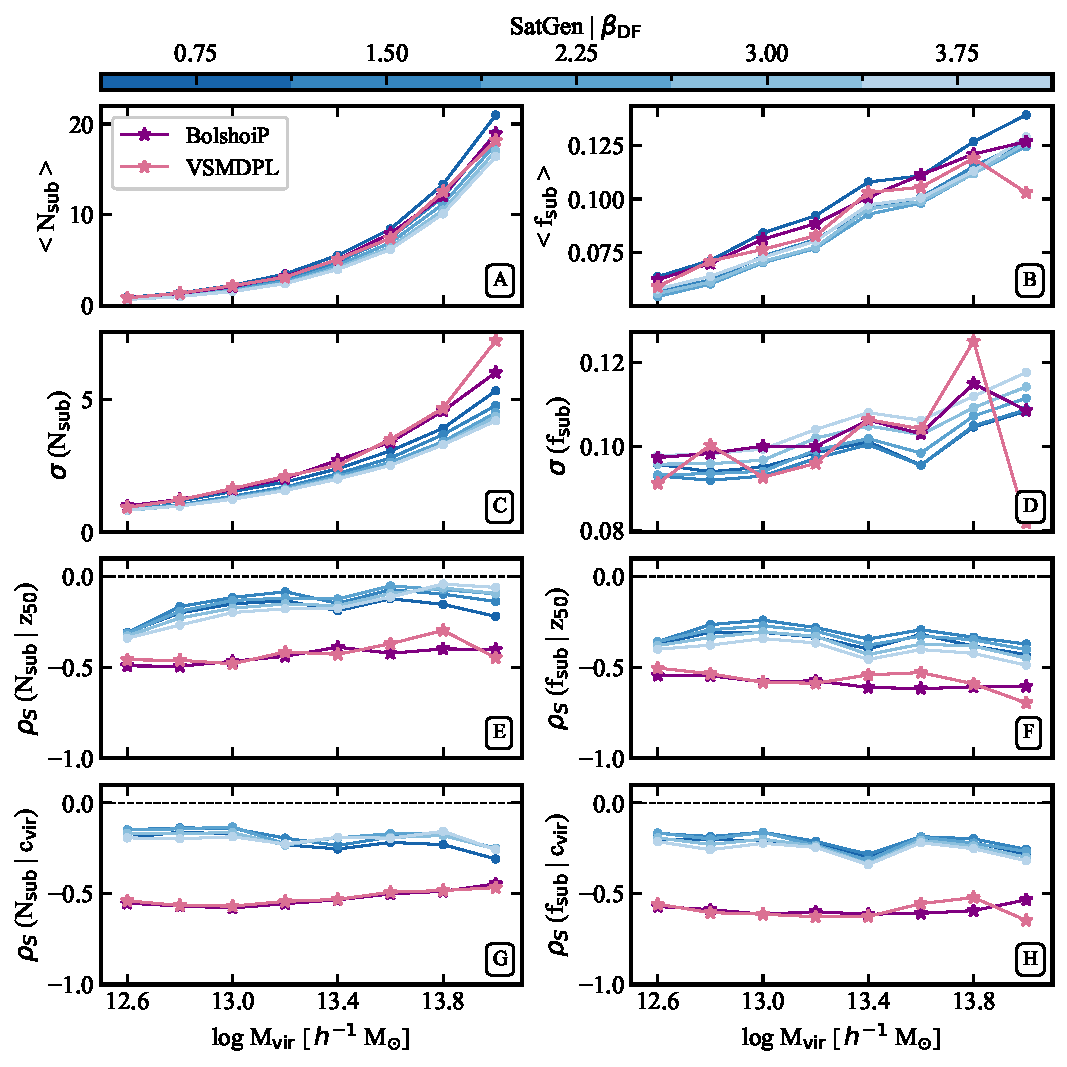
\includegraphics{paper/DF_full.pdf}
    \caption{The \SatGen\ models' HAB signal as a function of the strength of dynamical friction. Here the BolshoiP simulation is shown in purple and VSMDPL in pink but now the \SatGen\ model is colored by the assumed value of $\betadf$ as indicated. Our fiducial model $\betadf = 0.75$ corresponds to the darkest shade of blue, while the lightest shade corresponds to a 5x increase in the assumed strength of dynamical friction. The means of the $<\nsub>$ and $<\fsub>$ distributions (per host halo mass sample), are shown in Panels A and B, respectively. Similarly, the standard deviations of the $\sigma(\nsub)$ and $\sigma(\fsub)$ distributions, are shown in Panels C and D, respectively. We show the same correlation coefficients as in Figure \ref{fig:correlations} with $\rho_S(\nsub | \zfive)$ in panel E, $\rho_S(\fsub | \zfive)$ in panel F, $\rho_S(\nsub | \cvir)$ in panel G, and finally $\rho_S(\fsub | \cvir)$ in panel H. For clarity, the jack-knife errorbars were not plotted but are qualitatively the same as before. Notice that though $\betadf$ impacts the top four panels, it does not significantly change the measured HAB signal in the bottom four panels.}
    \label{fig:DF}
\end{figure*}

In this section we discuss one of the main parameters that governs the mass loss of subhalos in our semi-analytic framework and which can in principal be tuned to match simulations: the strength of dynamical friction. In the \SatGen\ model each subhalo is integrated in the potential of its direct parent, accounting for a dynamical friction force
%
\begin{equation}
F_{\rm DF}=-4 \pi \frac{G^2 m^2 }{v^2} \, \log{\Lambda} \, \rho(<v) \, \frac{v}{| v | } 
\end{equation}
%
\citep{Chandrasekhar.43}. Here, $m$ is the instantaneous subhalo mass, $\log \Lambda$ is the Coulomb logarithm, $v$ is the relative velocity of the subhalo with respect to its parent halo, and $\rho(<v)$ is the local density of dark matter particles in the parent halo with a speed less than $|v|$, which is computed under the standard assumption that the particles follow an isotropic Maxwellian velocity distribution \citep[see][]{Binney.Tremaine.08}. The Coulomb logarithm is modeled using
%
\begin{equation}\label{coulomb}
\log \Lambda= \betadf \, \log \left(M / m\right)\,,
\end{equation}
%
where $M$ is the instantaneous mass of the parent halo and $\beta_{\rm DF}$ is a free parameter that regulates the overall strength of dynamical friction. For comparisons to BolshoiP, \cite{Green.etal.21} found that $\beta_{\rm DF} = 0.75$ worked best at reproducing present-day radial distributions. \cite{Monzon.etal.26} instead adopted a fiducial value of $\beta_{\rm DF} = 1.0$ and showed how varying this parameter by a factor 2 does not significantly impact the \SatGen\ model's prediction for the accreted stellar halos around MW-like galaxies.

To investigate the impact of $\betadf$ on the HAB signal, we took the 8,000 trees described in Section $\ref{sec:DF}$ and reran our model's orbit integration step four more times, resulting in a set of five models with $\beta_{\rm DF} = [0.75, 1.5, 2.25, 3.00, 3.75]$. Because we reused the same merger trees, each host has identical $\zfive$ and $\cvir$ values across all five models. This means that changing $\betadf$ can alter the HAB signal only if its effect on the subhalo populations depends systematically on host assembly history—for example, if it preferentially modifies the subhalo populations of a subset of hosts within a given mass bin. We show the results of this test in Figure \ref{fig:DF} as a function of $\Mvir$.

As before, BolshoiP is shown in purple and VSMDPL in pink. Now the \SatGen\ model is colored by the assumed value of $\betadf$ as indicated. The means, $<\nsub>$ and $<\fsub>$, are shown in Panels A and B, respectively. Similarly, the standard deviations, $\sigma(\nsub)$ and $\sigma(\fsub)$, are shown in Panels C and D, respectively. The bottom four panels show the same rank-order correlation coefficients as in Figure \ref{fig:correlations}, but this time for each of the $\betadf$ models. Specifically, we show $\rho_S(\nsub | \zfive)$ in panel E, $\rho_S(\fsub | \zfive)$ in panel F, $\rho_S(\nsub | \cvir)$ in panel G, and finally $\rho_S(\fsub | \cvir)$ in panel H. 

The clear color gradients in Panels A and B show that, as expected, increasing $\betadf$ results in fewer, less massive subhalos. We can also see that, in terms of $<\nsub>$ and $<\fsub>$, our fiducial value of $\betadf$ is in good agreement with the MultiDark suite. The standard deviations $\sigma(\nsub)$ and $\sigma(\fsub)$ in Panels C and D show that our fiducial model slightly underpredicts the width of the distributions for higher values of $\Mvir$ and that increasing $\betadf$ has the opposite effect on $\sigma(\nsub)$ than it does on $\sigma(\fsub)$. This differing response is not necessarily unexpected, since $\nsub$ can be nicely approximated as a Poisson distribution \citep{Jiang.vdBosch.17}, but $\fsub$ depends not only on the number of surviving subhalos but also on their individual masses and correlations between their masses. Finally, the lack of clear color gradients in Panels E, F, G, and H shows that tuning this free parameter does not significantly impact the \SatGen\ model's HAB signal.

Because dynamical friction primarily impacts the orbits of systems with high merger ratios \citep{vdBosch.99}, only a subset of the overall subhalo population is strongly affected by changes in $\betadf$. Consequently, while changing $\betadf$ could produce a substantial effect on these hosts, its impact on the entire population is diluted by the larger fraction of hosts whose subhalo populations are largely insensitive to $\betadf$. In other words, while increasing $\betadf$ systematically shifts the normalization of $\nsub$ and $\fsub$ across the entire population, it does not significantly reshape the subhalo populations of hosts as a function of their particular assembly history.

Though $\betadf$ primarily controls the efficiency with which a subhalo's orbit decays and can shift the normalization of the surviving subhalo population, within our semi-analytic framework, it is not itself a significant driver of the HAB signal. This result is perhaps not unsurprising given that, in this experiment, varying $\betadf$ does not directly impact either the $\zfive$ or $\cvir$ distributions. This is because both distributions are set in the initial merger tree generation step and not in the subsequent orbit evolution step\footnote{Introducing a coupling between concentration, mass accretion histories, and our analytic prescription for dynamical friction would likely require iterating across both the merger tree generation and orbit evolution steps. This would introduce substantial computational overhead relative to our current pipeline and would require an empirically-derived convergence limit.}. Thus, this experiment tests whether changing orbital evolution at fixed assembly history can generate an additional HAB signal. The bottom four panels show that even a factor of 5 in the assumed value of $\betadf$ produces little change in the rank-order correlations between the surviving subhalo populations and either $\zfive$ or $\cvir$.

Another effect that might do so is related to the statistics of orbital infall. In the semi-analytical models, when a subhalo is accreted it is assigned an orbital energy and angular momentum (or, equivalently, a radial and tangential infall velocity), after which its orbit is integrated while accounting for dynamical friction and tidal effects. The orbital energy and angular momentum are drawn from universal distributions that carry no environment dependence. However, it is not difficult to envision a scenario in which, for example, the orbital eccentricity depends on the large scale tidal field. And since more radial orbits result in more stripping, everything else being equal, such an environmental dependence could once again impact the relation between formation history and subhalo abundance. Indeed, \citet{Shi.etal.15} found that the average tangential velocity increases with the strength of the tidal field in which the host halo resides, and that the distributions of both the radial and tangential infall velocities are broader in a stronger tidal environment. They also demonstrated that the internal velocity anisotropy of dark matter
halos are correlated with the strength of the tidal field in which it is embedded. Such dependencies have
thus far not been accounted for in semi-analytical models for the substructure of dark matter halos.
The main goal of this paper is to use one such model, \SatGen\, and to compare its detailed 

\jsm{The $\fsub$ and $\nsub$ rows were removed from Figure \ref{fig:scaling}, so this paragraph and the next need reworking (or should point to Figure \ref{fig:SHMF}).} The third row of Figure \ref{fig:scaling} shows that as $\Mvir$ increases, the fraction of mass contained in surviving subhalos, $\fsub$, also increases. This trend arises because more massive hosts assemble the bulk of material at later times, such that their subhalo populations are, on average, accreted more recently and have experienced less tidal stripping and disruption. In contrast, the subhalo populations of lower-mass hosts were generally accreted earlier, providing more time for tidal forces and dynamical friction to reduce their masses or disrupt them entirely. Notice how our choice of $\mthresh$ causes an absence of colored points below the mean lines in the third row for $\Mvir \lesssim 10^{13.2} \Msunh$ because $\fsub$ is measured relative to $\mthresh$ (see Equation \ref{eq:fsub}). Here, our fiducial version of the \SatGen\ model seems to slightly over-predict $\fsub$ relative to the simulations. That being said, given the significant scatter in the $\fsub$ and $\Mvir$ relation, a linear fit is not very illuminating \citep{Jiang.vdBosch.16}.

Finally, the bottom row of Figure~\ref{fig:scaling} shows subhalo abundance at present-day. Notice how our choice of $\mthresh$ causes $\log \nsub$ to scale almost linearly with $\log \Mvir$ such that $\nsub \approx 1$ for the $\mathbb{S}_{12.6}$ sample and $\nsub \approx 30$ for the $\mathbb{S}_{14.0}$ sample. Here again, the \SatGen\ model seems to slightly over-predict the $\nsub$ and $\Mvir$ relation. 

Notice that by virtue of being a smaller cosmological volume (see Table \ref{tab:sims}), the SHMFs in VSMDPL become slightly noisier as the number of hosts in each mass sample decreases.

%%%%%%
Removed from main.tex by Claude, 2026-11-17/18 (restored here, verbatim)
%%%%%%

% Sec 3.1, Overleaf version of the Fig. 2 sentence dropped when resolving the 2026-11-17 merge conflict
Figure~\ref{fig:scaling} shows scaling relations for all host halo properties related to assembly history. From top to bottom, the different rows show $\zfive$, $\cvir$, $\fsub$ and $\nsub$.


%%%%%% moved from main.tex Section 4.2 (sec:ludlow) on 2026-11-18, per your note: "not sure we need this paragraph - maybe we save it for the discussion"

\jsm{To determine whether this improvement arises from subhalos evolving differently in the \cite{Ludlow.etal.16} host potential, we correlate the subhalo populations of the fiducial run with the \cite{Ludlow.etal.16} concentrations of the same trees. This yields nearly identical values (a concentration channel of $-0.20$ for $\nsub$ and $-0.16$ for $\fsub$), indicating that the improvement is not due to changes in the subhalo populations. Instead, because it depends on all progenitors through the CMH rather than on the main branch alone, the \cite{Ludlow.etal.16} concentration is simply a better summary of the assembly history of each tree. Even so, the concentration channel remains only about half as strong as in BolshoiP.}
